\subsection{Transcriptional Changes of Human \textit{IFITs}} \label{Transcriptional Changes of Human IFITs}
To unravel the impact of cellular stimulation with activators of the innate immune response and human RSV, on the expression of human \textit{IFIT} genes, quantitative real-time reverse transcription PCR (qPCR) analysis was executed in accordance with the methodology outlined in Section \ref{Quantitative Real Time/Reverse Transcription PCR}. Briefly, cells were cultivated in 12-well plates and subsequently subjected to the respective stimulants. At the endpoint of the experiments, the RNA was extracted, followed by cDNA synthesis and the transcript quantification by qPCR. All transcript levels were standardized to human \textit{GAPDH} expression, employing  the 
\(\Delta\)\(\Delta\)Ct method. Subsequently, all values were normalized against mock-treated samples, enabling data aggregation and inter-experimental induction value comparison. The statistical analysis was conducted as outlined in Section \ref{Statistical Analysis}. Notably, the choice of the appropriate statistical test hinged on the normality of data distribution and equality of variance, aspects which will be underscored in the ensuing text.



\subsubsection{Human \textit{IFITs} Responses of to Known Activators of Innate Immune Response} \label{Human IFIT Responses to Known Activators of Innate Immune Response}
In order to establish the expression competency of human \textit{IFITs} of the A549 cell line, along with elucidating how different innate immune pathways contribute to the overall expression profile, I treated the cells with differing activators of the innate immune response. As described in Section \ref{Routes of IFIT Expression Activation}, and depicted in Figure \ref{Pathways Inducing ISG mRNA Production.},  interferon-stimulated genes (ISGs) can have their induction activated either via the interferon receptor signalling, intracellular foreign nucleic acid detection or via extracellular PAMP sensing. The latter, in the context of RSV, includes stimulation of TLR4 with either LPS or RSV particles. After surveying the literature I ended up using 1,000 international units (IU) per mL of human interferon alpha (\cite{Terenzi2006DistinctISG56}; \cite{Santhakumar2018ChickenViruses}). For interferon-gamma stimulation, which stimulates predominantly immune cells \textit{in vivo} concentrations of 500, 1,000 and 2,000 IU/mL were used. LPS was administered in concentrations of 5 ng/mL and 5 \(\mu\)g/mL for the duration of 6 hours. (\cite{Mears2019Ifit1Cells}; \cite{Zhang2019GrouperResponse}). To stimulate intracellular foreign nucleic acid recognition 2 \(\mu\)g of poly I:C were transfected into A549 cells and incubated for 24 hours (\cite{Mears2019Ifit1Cells}; \cite{Palchetti2015TransfectedCells}).

\begin{figure}
    \centering
    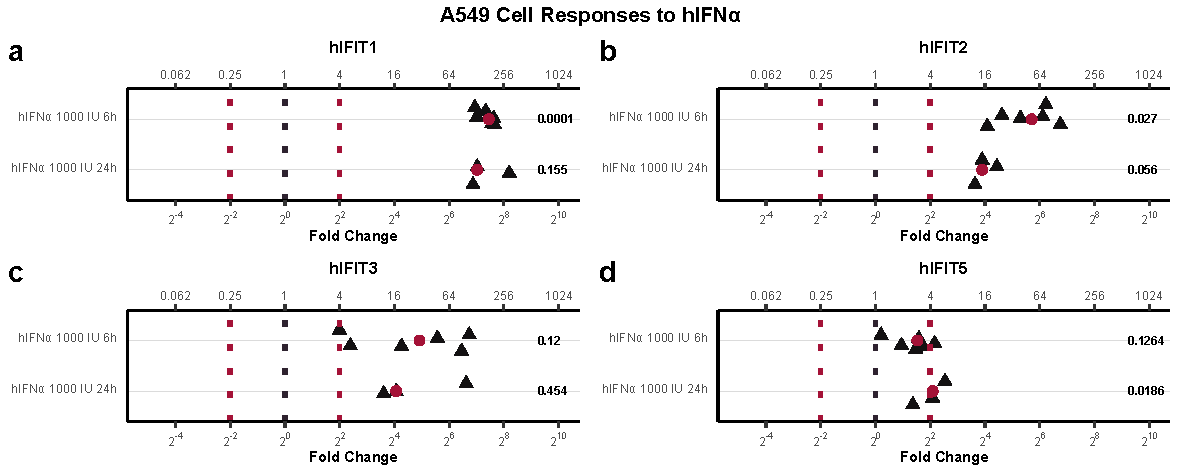
\includegraphics[width=1\linewidth]{06. Chapter 1/Figs/01. Induction/01. a549_treat_ifna.pdf}
    \caption[qPCR Analysis of A549 \textit{hIFIT} Response to hIFN\(\alpha\).]{\textbf{qPCR Analysis of A549 \textit{hIFIT} to hIFN\(\alpha\).} The relative abundance of (a) \textit{hIFIT1}, (b) \textit{hIFIT2}, (c) \textit{hIFIT3}, and (d) \textit{hIFIT5} genes, extracted from the A549 cell line, with response to human interferon alpha (IFN\(\alpha\)) at a concentration of 1000 IU per mL for a treatment duration of 6 or 24 hours. The shown values are relative to standardised mock values. The red circles signify median values. The black dotted line indicates mock expression, while the red dotted lines indicate biologically significant levels of induction. Numeric values signify the p-values compared to mock.}
    \label{A549 Response to hIFNa}
\end{figure}

The A549 cell line, derived from   lung carcinomatous tissue from a 58-year-old Caucasian male in 1972 is a well-established model of alveolar epithelial cells, routinely used for cancer to viral research alike (\cite{Lieber1976ACells}). We observe that after the stimulation of the A549 cell line with 1,000 IU/mL of hIFN\(\alpha\) for either 6 or 24 hours human \textit{IFIT1}, \textit{IFIT2}, and \textit{IFIT3} were induced drastically, especially \textit{IFIT1}, which was induced around 200-fold (Figure \ref{A549 Response to hIFNa}). The relative induction levels were identical between \textit{IFIT2} and \textit{IFIT3}. For all of these 3 genes, we can observe a decreased expression with longer incubation of IFN\(\alpha\), i.e. approximately half of the induction levels caused by 6-hour long incubation. Human \textit{IFIT5} shows minimal induction compared to the other \textit{IFITs} (3 and 4-fold for 6 and 24-hour long incubation respectively), which hovers around the mark of what is considered biologically significant induction, especially for ISGs, which are supposed not to be highly basally expressed. We can also observe a reverse trend of the time dependency of hIFN\(\alpha\)-induced expression. This suggests differential induction sensitivities between \textit{hIFIT1} (highly induced), \textit{hIFIT2} and \textit{hIFIT3} (medium induced) and \textit{hIFIT5} (low induced). All \textit{hIFIT} values had normal distributions and unequal variance other than \textit{hIFIT5}, which had normal distribution and normal variance.

\begin{figure}
    \centering
    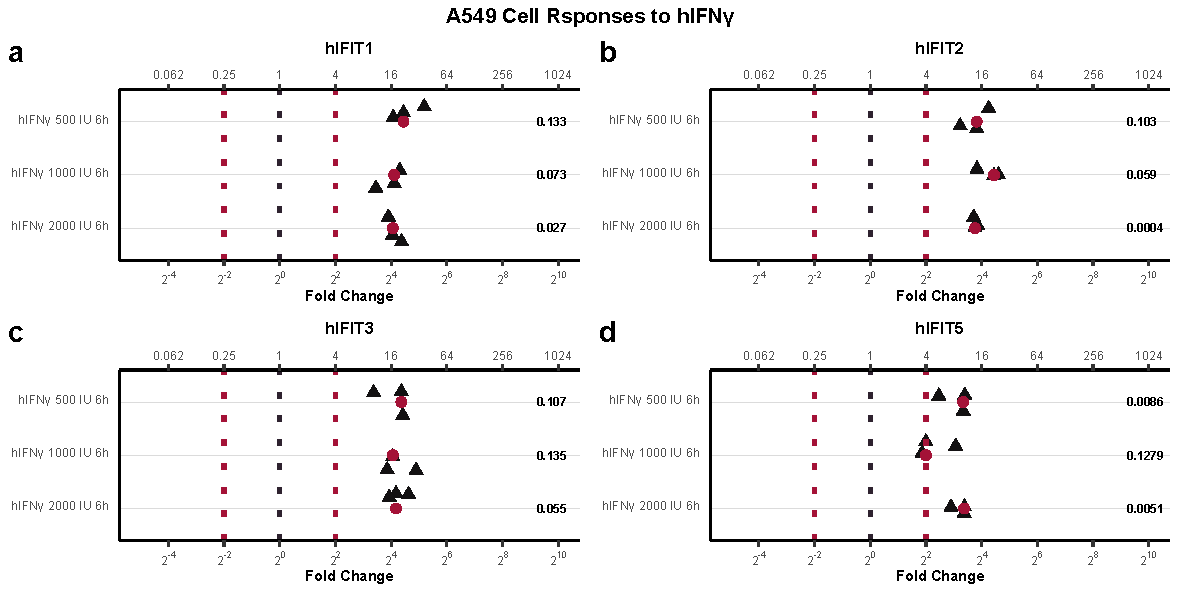
\includegraphics[width=1\linewidth]{06. Chapter 1/Figs/01. Induction/02. a549_treat_ifng.pdf}
    \caption[qPCR Analysis of A549 \textit{hIFIT} Response to hIFN\(\gamma\).]{\textbf{qPCR Analysis of A549 \textit{hIFIT} Response to hIFN\(\gamma\).} The relative abundance of (a) \textit{hIFIT1}, (b) \textit{hIFIT2}, (c) \textit{hIFIT3}, and (d) \textit{hIFIT5} genes, extracted from the A549 cell line, with response to human interferon-gamma (IFN\(\gamma\)) at concentrations of 500, 1000, and 2000 IU per mL for a treatment duration of 6 hours. The shown values are relative to standardised mock values. The red circles signify median values. The black dotted line indicates mock expression, while the red dotted lines indicate biologically significant levels of induction. Numeric values signify the p-values compared to mock.}
    \label{A549 Response to hIFNg}
\end{figure}

The response of human \textit{IFIT} genes to human IFN gamma can be seen in Figure \ref{A549 Response to hIFNg}. We can observe all \textit{IFITs} other than \textit{hIFIT5} responding equally to all concentrations tested i.e. 500, 1,000 and 2,000 IU/mL. Their response was concentration independent of a magnitude of around 15-fold. \textit{hIFIT5} response to very low concentration and very high concentrations was around 10-fold, while its transcript abundance increased only 4 times when treated with 1,000 IU/mL concentration. This suggests that the interferon-gamma component of the human \textit{IFIT} response is relatively equal for all of the \textit{IFIT} genes. This data, along with the data from hIFN\(\alpha\) induction also confirms that the A549 cell line is \textit{hIFIT} induction capable, which is great. All \textit{hIFIT} values had normal distributions and unequal variance other than \textit{hIFIT5}, which had normal distribution and normal variance.

\begin{figure}
    \centering
    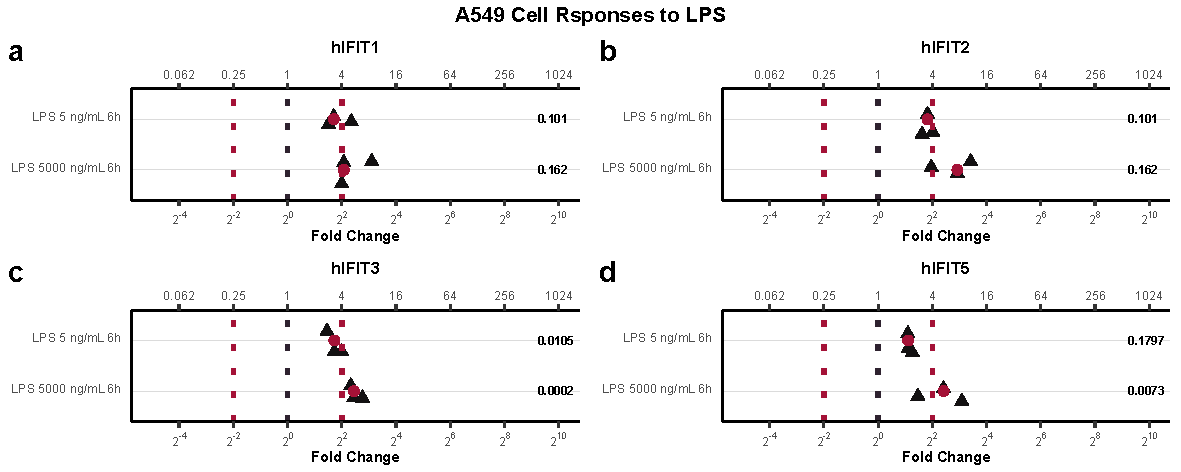
\includegraphics[width=1\linewidth]{06. Chapter 1/Figs/01. Induction/03. a549_treat_lps.pdf}
    \caption[qPCR Analysis of A549 \textit{hIFIT} Response to LPS.]{\textbf{qPCR Analysis of A549 \textit{hIFIT} Response to LPS.} The relative abundance of (a) \textit{hIFIT1}, (b) \textit{hIFIT2}, (c) \textit{hIFIT3}, and (d) \textit{hIFIT5} genes, extracted from the A549 cell line, with response to lipopolysaccharide (LPS) at concentrations of 5 and 5000 ng/mL for a treatment duration of 6 hours. The shown values are relative to standardised mock values. The red circles signify median values. The black dotted line indicates mock expression, while the red dotted lines indicate biologically significant levels of induction. Numeric values signify the p-values compared to mock.}
    \label{A549 Response to LPS}
\end{figure}

In order to assess the involvement of TLR4, a receptor also responsible for detecting RSV particles, A549 cells were incubated for 6 hours with low (5 ng/mL) and high (5,000 ng/mL) concentrations of bacterial LPS, its known activator. We can see that all \textit{IFITs} respond in a concentration dependant manner but the response is the lowest out of the different stimulants used. Low-concentration LPS incubation causes biologically insignificant induction of all \textit{hIFITs} of 2-fold for \textit{hIFIT5} and 3-fold for the other \textit{IFITs}. The high concentration on the other hand yields biologically significant induction levels of 4-8 fold induction. All \textit{hIFIT} values had normal distributions and unequal variance other than \textit{hIFIT3}, which had normal distribution and normal variance.

\begin{figure}
    \centering
    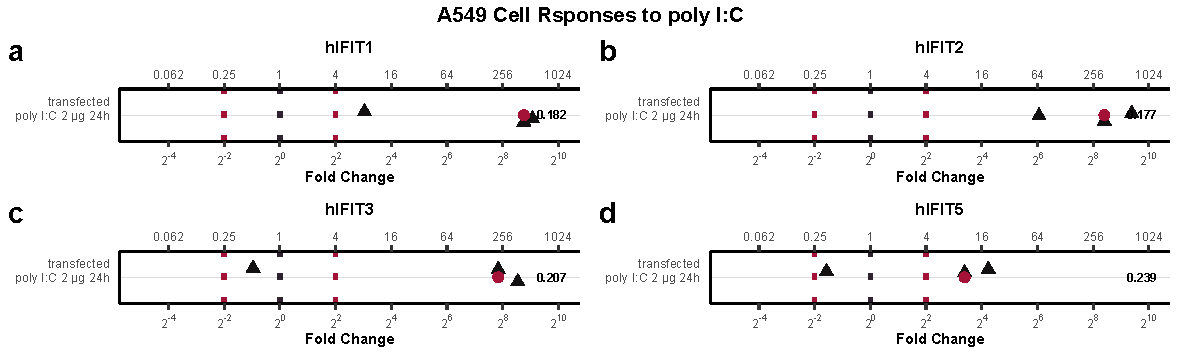
\includegraphics[width=1\linewidth]{06. Chapter 1/Figs/01. Induction/04. a549_treat_polyic.pdf}
    \caption[qPCR Analysis of A549 \textit{hIFIT} Response to Transfected poly I:C.]{\textbf{qPCR Analysis of A549 \textit{hIFIT} Response to Transfected poly I:C.} The relative abundance of (a) \textit{hIFIT1}, (b) \textit{hIFIT2}, (c) \textit{hIFIT3}, and (d) \textit{hIFIT5} genes, extracted from the A549 cell line. The cells were transfected with 2 \(\mu\)g of poly I:C for 24 hours. The shown values are relative to standardised mock values. The red circles signify median values. The black dotted line indicates mock expression, while the red dotted lines indicate biologically significant levels of induction. Numeric values signify the p-values compared to mock.}
    \label{A549 Response to poly I:C}
\end{figure}

When A549 cells were transfected with 2\(\mu\)g of poly I:C for 24 hours we were able to observe the biggest induction compared to the other inducers previously used (Figure \ref{A549 Response to poly I:C}). As with the other inducers, hIFIT1 induction is the greatest (circa 500-fold), followed by \textit{hIFIT2} and \textit{hIFIT3} with 300-fold and 200-fold responses respectively, with \textit{hIFIT5} trailing behind with the lowest response of only 10-fold. This again suggests that \textit{hIFIT5} seems to have differential transcriptomic regulation compared to the other genes of the \textit{IFIT} family. All \textit{hIFIT} values had normal distributions and unequal variance.

\begin{figure}
    \centering
    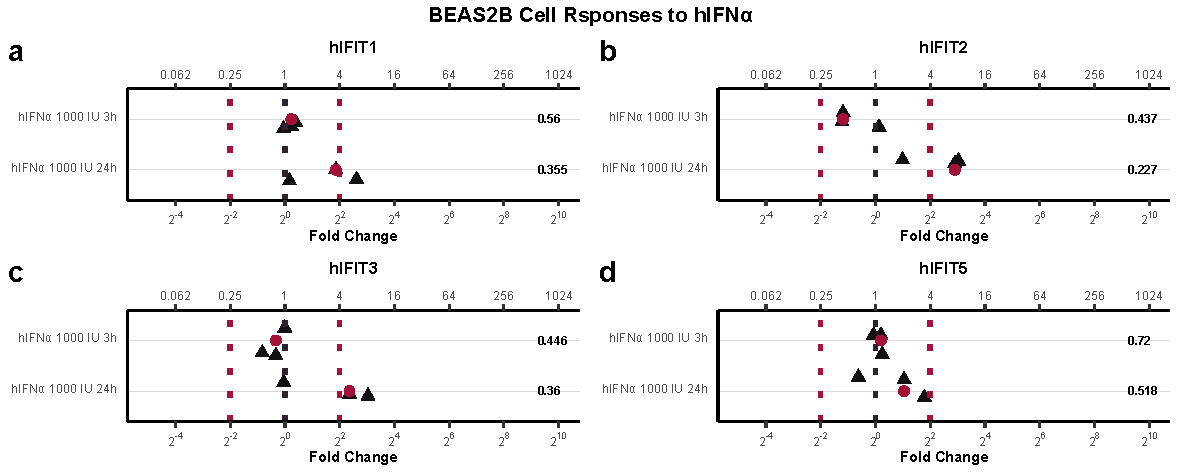
\includegraphics[width=1\linewidth]{06. Chapter 1/Figs/01. Induction/09. beas2b_ifna.pdf}
    \caption[qPCR Analysis of BEAS-2B \textit{hIFIT} Response to hIFN\(\alpha\).]{\textbf{qPCR Analysis of BEAS-2B \textit{hIFIT} Response to hIFN\(\alpha\).} The relative abundance of (a) \textit{hIFIT1}, (b) \textit{hIFIT2}, (c) \textit{hIFIT3}, and (d) \textit{hIFIT5} genes, extracted from the BEAS-2B cell line, with response to human interferon alpha (IFN\(\alpha\)) at a concentration of 1000 IU per mL for a treatment duration of 3 or 24 hours. The shown values are relative to standardised mock values. The red circles signify median values. The black dotted line indicates mock expression, while the red dotted lines indicate biologically significant levels of induction. Numeric values signify the p-values compared to mock.}
    \label{BEAS-2B responses to hIFNa}
\end{figure}

Lastly, we validated the human interferon alpha induction data in a more biologically relevant cell line, BEAS-2B. Established from bronchial epithelial biopsies from healthy samples, and later immortalised using the transfection of cyclin-dependent kinase 4 and human telomerase reverse transcriptase, these cells are an invaluable tool in the field of bronchial development and pathogenesis (\cite{Ramirez2004ImmortalizationOncoproteins}). After the treatment with human interferon alpha at concentrations of 1,000 IU/mL for 3 hours, we can see that this stimulation was not sufficient to induce the expression of any human \textit{IFIT} (Figure \ref{BEAS-2B responses to hIFNa.}). However, when the cells were stimulated for 24 hours we can observe induction above biological significance for \textit{hIFIT1}, \textit{hIFIT2}, and \textit{hIFIT3}, with 4-fold, 8-fold, and 5-fold increase respectively. \textit{hIFIT5} shows only 2-fold median induction, which could be caused by the intrinsic variability of the assay. So as we observed with the A549 cell line, \textit{hIFIT5} behaves in discord with the other human \textit{IFITs}. All \textit{hIFIT} values had normal distributions and unequal variance.


\subsubsection{Human \textit{IFITs} Responses to hRSV} \label{Human \textit{IFITs} Responses to hRSV}
Old text:
In line with bovine IFIT responses investigation, human IFIT responses to human (h) RSV were assessed. The virus was prepared as described in section 7.1. Briefly, infected cells were sonicated, cell debris was separated by centrifugation and virus-containing supernatant was gathered and titred. Human epithelial type 2 (HEp-2) cells were infected with the hRSV-containing supernatant at multiplicities of infection (MOI) of 0.1 and 2. These cells were chosen for the initial preliminary experiments as they are known to grow the virus well and their tissue of origin (laryngeal carcinoma) is relevant to the native site of RSV replication. It is to be noted that this cell line is believed to be contaminated by HeLa cell line and in later experiments should be replaced by more physiological models of human lung epithelial tissue. As a positive control, 1000 U of hIFNα was used. Samples were collected 24 hours post-infection. Cellular RNA was extracted and converted to complementary DNA, as described in section 7.3. Human IFIT transcripts were quantified relative to mock-infected cells. GAPDH-normalised qPCR data can be seen in Figure 8. We observed no significant IFIT induction at the MOI of 0.1, however, infection with hRSV at an MOI of 2 provided significant induction for all targets tested. All human IFITs were induced by approximately 5-fold. With regards to interferon responses, all four targets were transcriptionally upregulated following IFNα treatment. The induction of hIFIT2 was equal to the one induced by viral infection at an MOI of 2, while the rest of hIFITs were induced more greatly. Compared to data described in section 8.3 here the variation was minimal and thus the data is more reliable. We can conclude that both interferon-alpha treatment, as well as RSV infection, transcriptionally upregulate human IFITs in HEp-2 cells.

How were viruses harvested and cells infected \newline
Justify moi and timepoints \newline
Justify uv inactivated virus and how it was done \newline

Describe data: \newline
asdasdasd \newline
UV inactivated RSV does not induce IFIT expression, meaning IFITs do not get activated by TLR4 detection of viral particles on the cell surface. Low MOI infection (0.1 MOI) does not induce IFITs. Infection at MOI 1 and 2 induce all IFITs regardless of the length of infection (24 and 48 HPI). The purification methodology for virus extraction (ultra purification on sucrose cushion vs just clearing the cells + supernatant by centrifugation) does not influence IFIT induction.



\begin{figure}
    \centering
    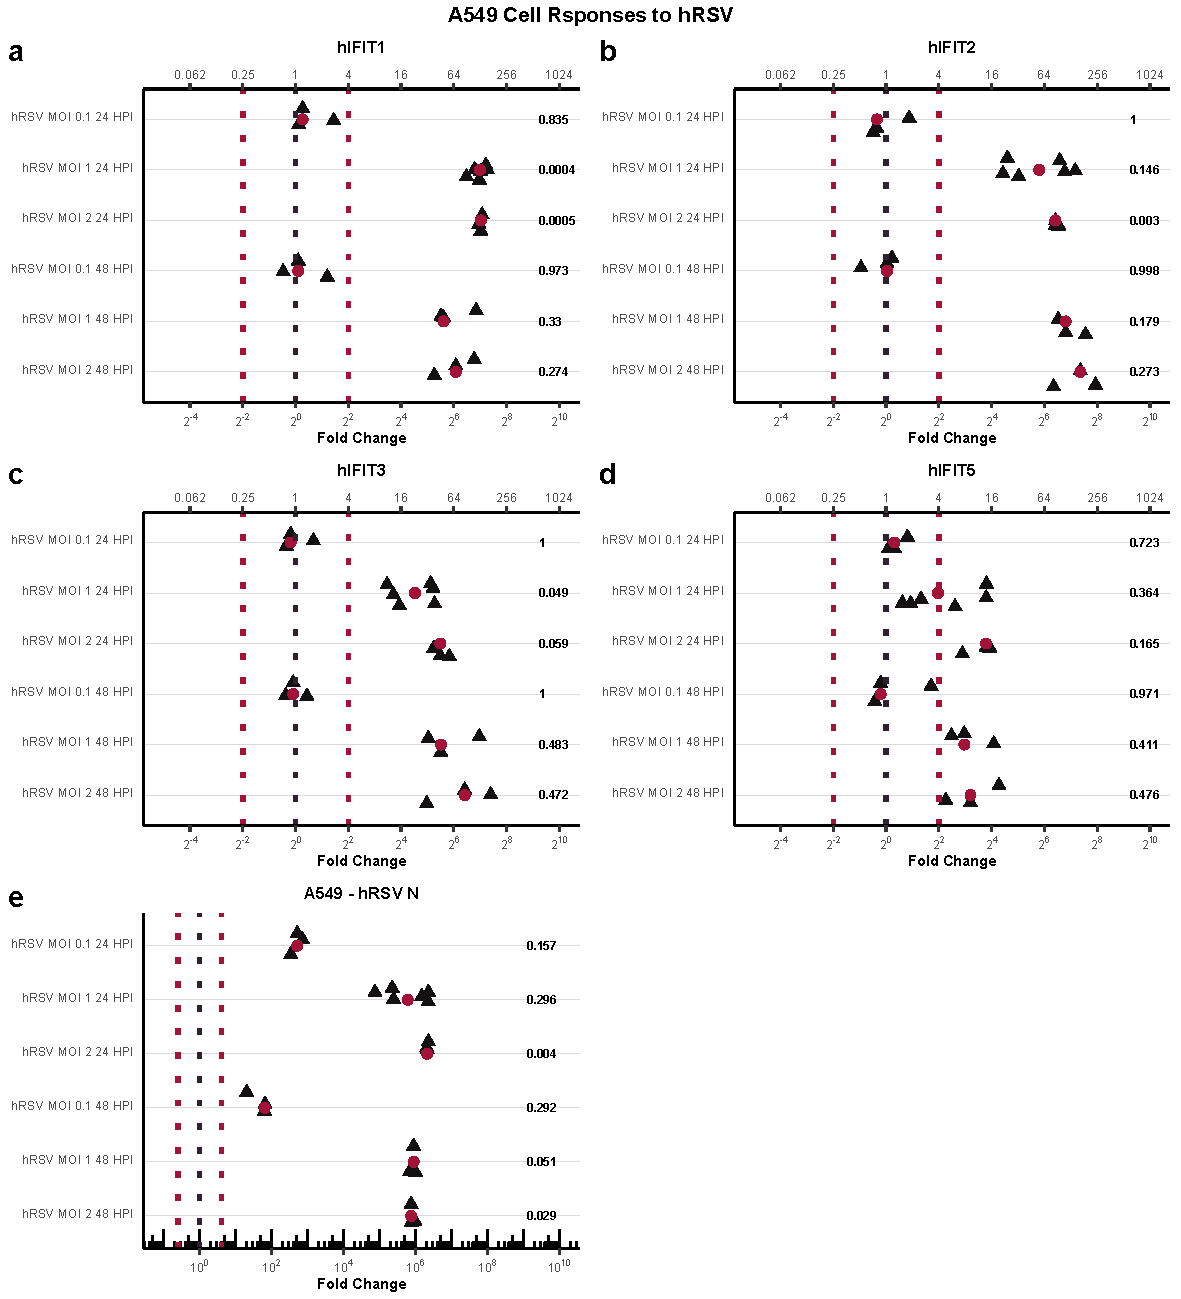
\includegraphics[width=1\linewidth]{06. Chapter 1/Figs/01. Induction/05. a549_hrsv_timepoints.pdf}
    \caption[A549 \textit{hIFIT} Response to hRSV asa Function of Time and MOI.]{\textbf{A549 \textit{hIFIT} Response to hRSV asa Function of Time and MOI.} The relative abundance of (a) \textit{hIFIT1}, (b) \textit{hIFIT2}, (c) \textit{hIFIT3}, (d) \textit{hIFIT5} and (e) \textit{hRSV N} genes, extracted from A549 cell line following infection with human RSV at MOI of either 0.1, 1, or 2 for either 24 or 48 hours post-infection. The shown values are relative to standardised mock values. The red circles signify median values. The black dotted line indicates mock expression, while the red dotted lines indicate biologically significant levels of induction. Numeric values signify the p-values compared to mock.}
    \label{A549 response to hRSV timepoints}
\end{figure}

some text between these two suckers that will say about how the human ifit induction is dependent on replication and interferon.

\begin{figure}
    \centering
    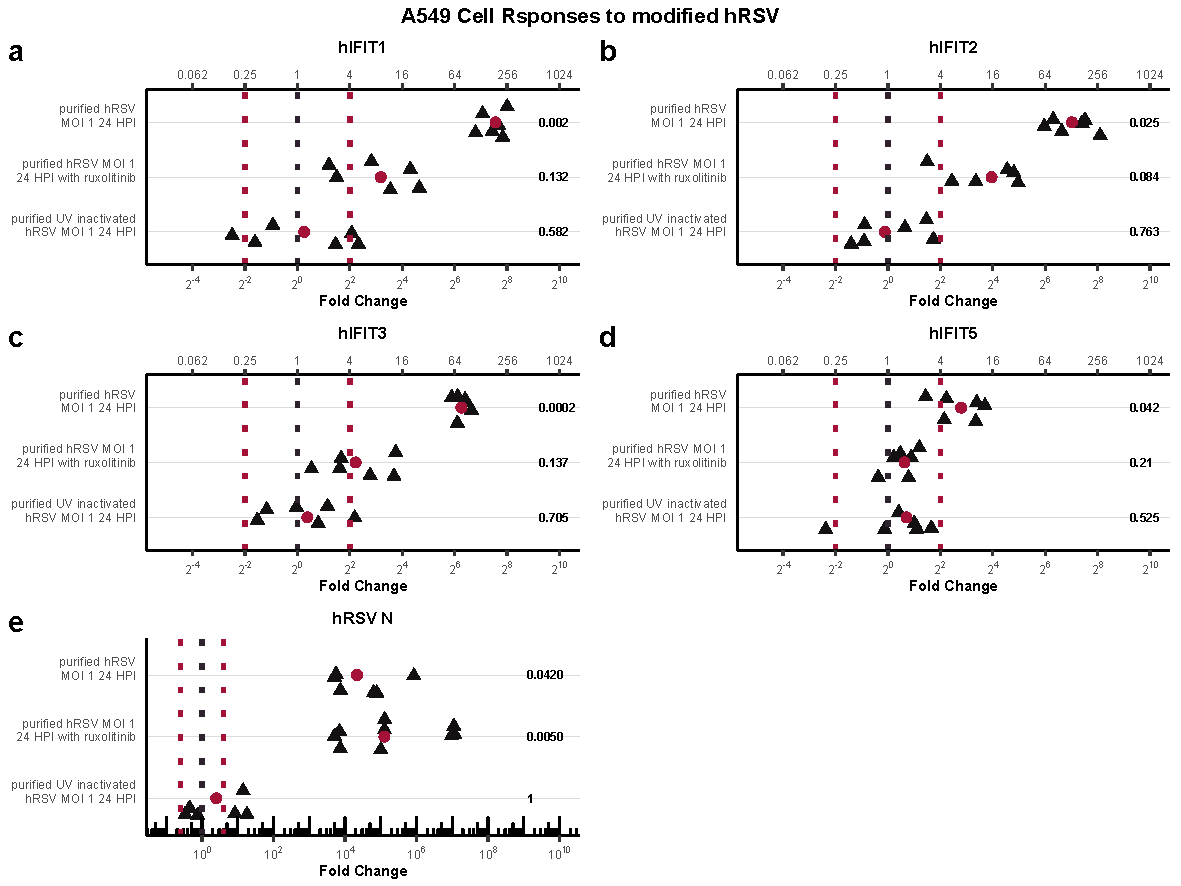
\includegraphics[width=1\linewidth]{06. Chapter 1/Figs/01. Induction/06. a549_hrsv_uv_roxo.pdf}
    \caption[The Effect of Ultra-Purification, UV-Inactivation and INFR Inhibition on \textit{hIFIT} Induction Following hRSV Infection.]{\textbf{The Effect of Ultra-Purification, UV-Inactivation and INFR Inhibition on \textit{hIFIT} Induction Following hRSV Infection.} The relative abundance of (a) \textit{hIFIT1}, (b) \textit{hIFIT2}, (c) \textit{hIFIT3}, (d) \textit{hIFIT5} and (e) \textit{hRSV N} genes, extracted from A549 cell line following infection with ultra-purified hRSV at MOI 1 for 24 hours. The cells were either treated with the virus alone (first row), or with the virus and 5 nM of ruxolitinib (interferon receptor inhibitor) during the whole infection period (second row), or with UV-inactivated hRSV (last row). The shown values are relative to standardised mock values. The red circles signify median values. The black dotted line indicates mock expression, while the red dotted lines indicate biologically significant levels of induction. Numeric values signify the p-values compared to mock.}
    \label{The effect of ultra-purification, UV-inactivation and INFR inhibition on hIFIT induction following hRSV infection}
\end{figure}

\begin{figure}
    \centering
    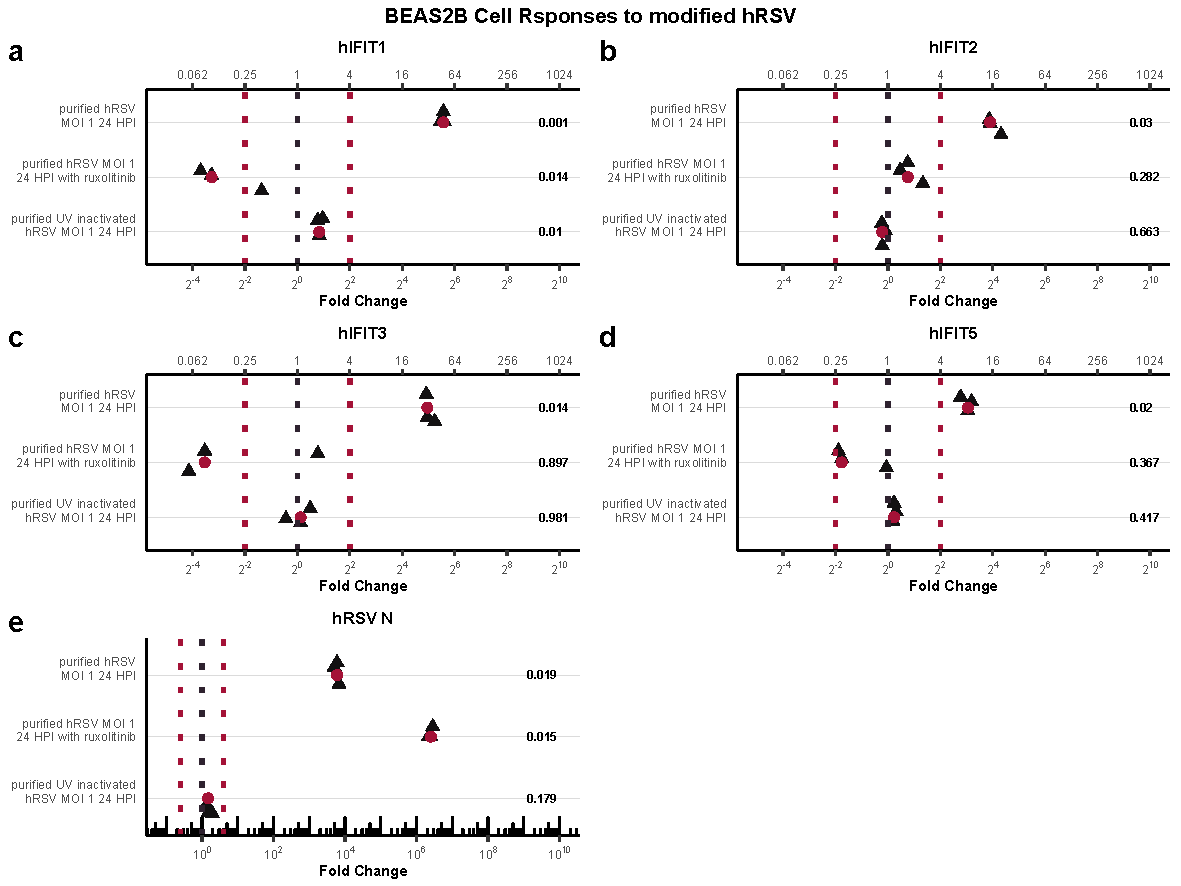
\includegraphics[width=1\linewidth]{06. Chapter 1/Figs/01. Induction/10. beas2b_hrsv.pdf}
    \caption[BEAS-2B responses to hRSV.]{BEAS-2B responses to hRSV.}
    \label{BEAS-2B responses to hRSV.}
\end{figure}



Describe data: \newline
asdasdasd \newline
Validation in more physiologically relevant cell line. UV inactivated hRSV does not cause induction. Ultracentrifugation purified hRSV causes induction in all IFITs. All IFITs but IFIT5 are induced by IFN alpha, but only after incubation for 24 hours (3h incubation does not cause induction). This shows that the cells are interferon competent. IFIT5 does not get induced by any bRSV infection tried (probably because IFIT5 has either basally higher levels and thus the same end mRNA concentration equates to lower induction or because it is really not induced by bRSV (although the IFITs should have the same promoters)). Low MOI infection (0.001 and 0.01) of dNS1 and dNS2 bRSV induces IFITs 1,2 and 3, while dSH MOI1 and dNS1/2 MOI 0.001 does not. 

The trends seen with A549 are kind of recapitulated.
\subsubsection{Validation by Comparing to the Proteomic Dataset} \label{Validation by Comparing to the Proteomic Dataset}
Who, what and why it was done  \newline
Cite the bioArchive paper \cite{Jobe2023ViralCondensates}

\begin{figure}
    \centering
    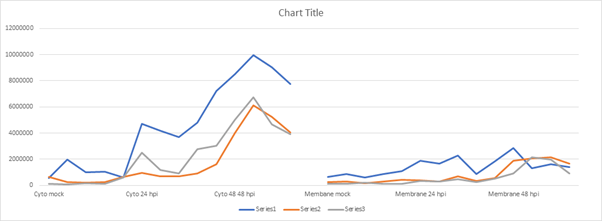
\includegraphics[width=1\linewidth]{06. Chapter 1/Figs/01. Induction/13. proteomics.png}
    \caption[Human IFIT proteins detected per fraction.]{\textbf{Human IFIT proteins detected per fraction.} test test test test test test test test test test test.}
    \label{Human IFIT proteins detected per fraction.}
\end{figure}

Describe data: \newline
asdasdasd \newline
Proteomics dataset from Dalan’s lab looking at differential enrichment of proteins between membrane and cytosolic fractures. It confirms that in A549 (I think) IFITs 1 (series 1), 2 (series 2) and 3 (series 3) are induced in the cytosolic fraction at protein level 

\subsubsection{Human \textit{IFITs} Responses to bRSV} \label{Human IFITs Responses to bRSV}
How were viruses harvested and cells infected \newline
Justify moi and timepoints

\begin{figure}
    \centering
    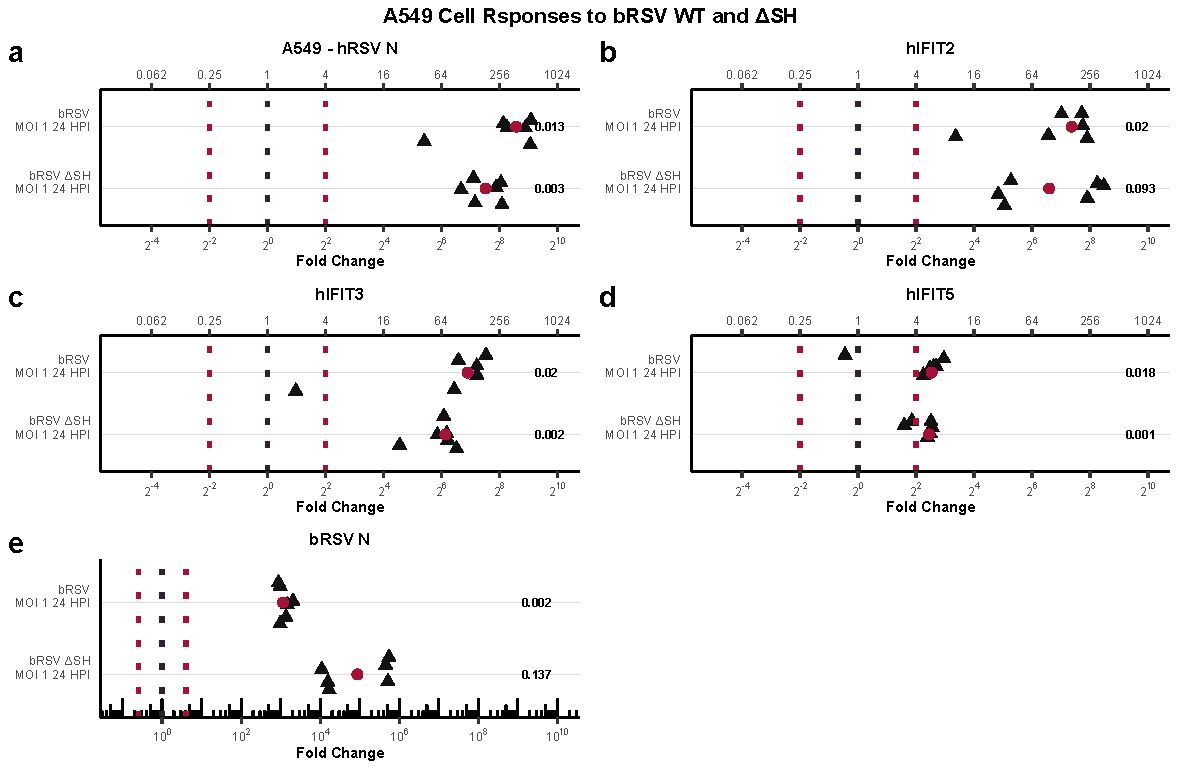
\includegraphics[width=1\linewidth]{06. Chapter 1/Figs/01. Induction/07. a549_brsv_moi1.pdf}
    \caption[Responses of A549 to bRSV WT and dSH.]{\textbf{Responses of A549 to bRSV WT and dSH.} Some filler text afterwards to not to forget.}
    \label{Responses of A549 to bRSV WT and dSH.}
\end{figure}

Describe data: \newline
asdasdasd \newline
Infection cells with WT bRSV induces IFITs more than infection with hRSV.  Infection with mutant bRSV viruses (at normal and low MOI) induces human IFITs but IFIT5, which is only responsive to MOI 1 dSH bRSV and MOI 0.001 dNS1/2 bRSV.

The low MOI infection causing induction are interesting as low MOI hRSV did not cause induction. Maybe bRSV is more potent of A549 cells?

\begin{figure}
    \centering
    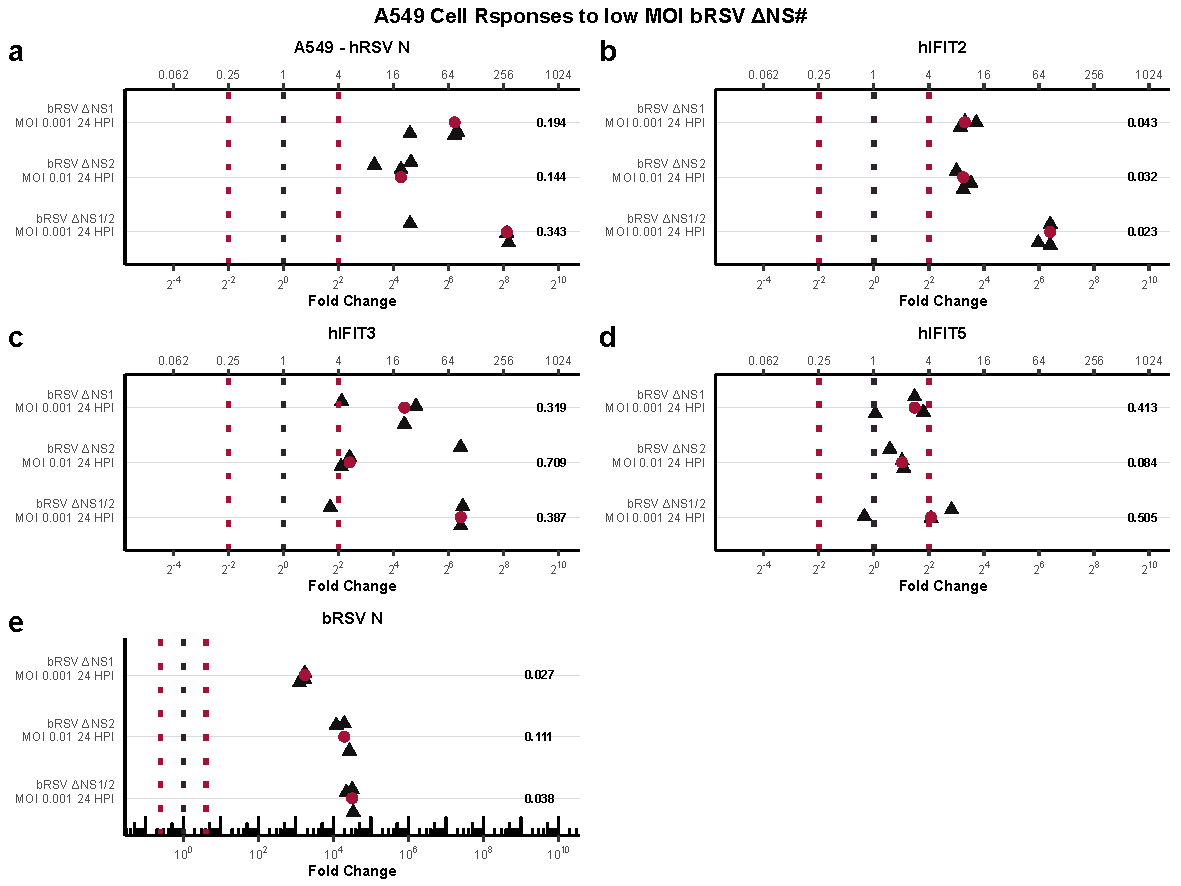
\includegraphics[width=1\linewidth]{06. Chapter 1/Figs/01. Induction/08. a549_brsv_dns.pdf}
    \caption[Responses of A549 to bRSV dNSs.]{\textbf{Responses of A549 to bRSV dNSs.} Some filler text afterwards to not to forget.}
    \label{Responses of A549 to bRSV dNSs.}
\end{figure}

\begin{figure}
    \centering
    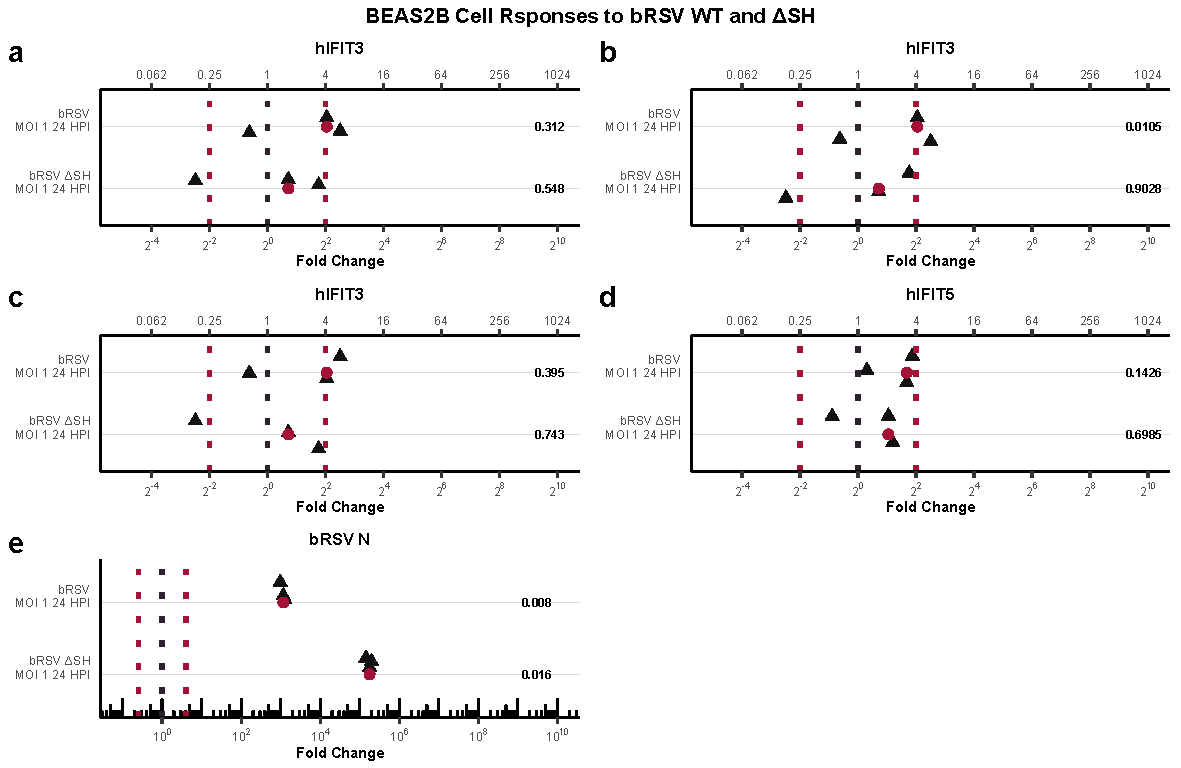
\includegraphics[width=1\linewidth]{06. Chapter 1/Figs/01. Induction/11. beas2b_brsv_moi1.pdf}
    \caption[BEAS-2B responses to bRSV WT and dSH.]{BEAS-2B responses to bRSV WT and dSH.}
    \label{BEAS-2B responses to bRSV WT and dSH.}
\end{figure}

\begin{figure}
    \centering
    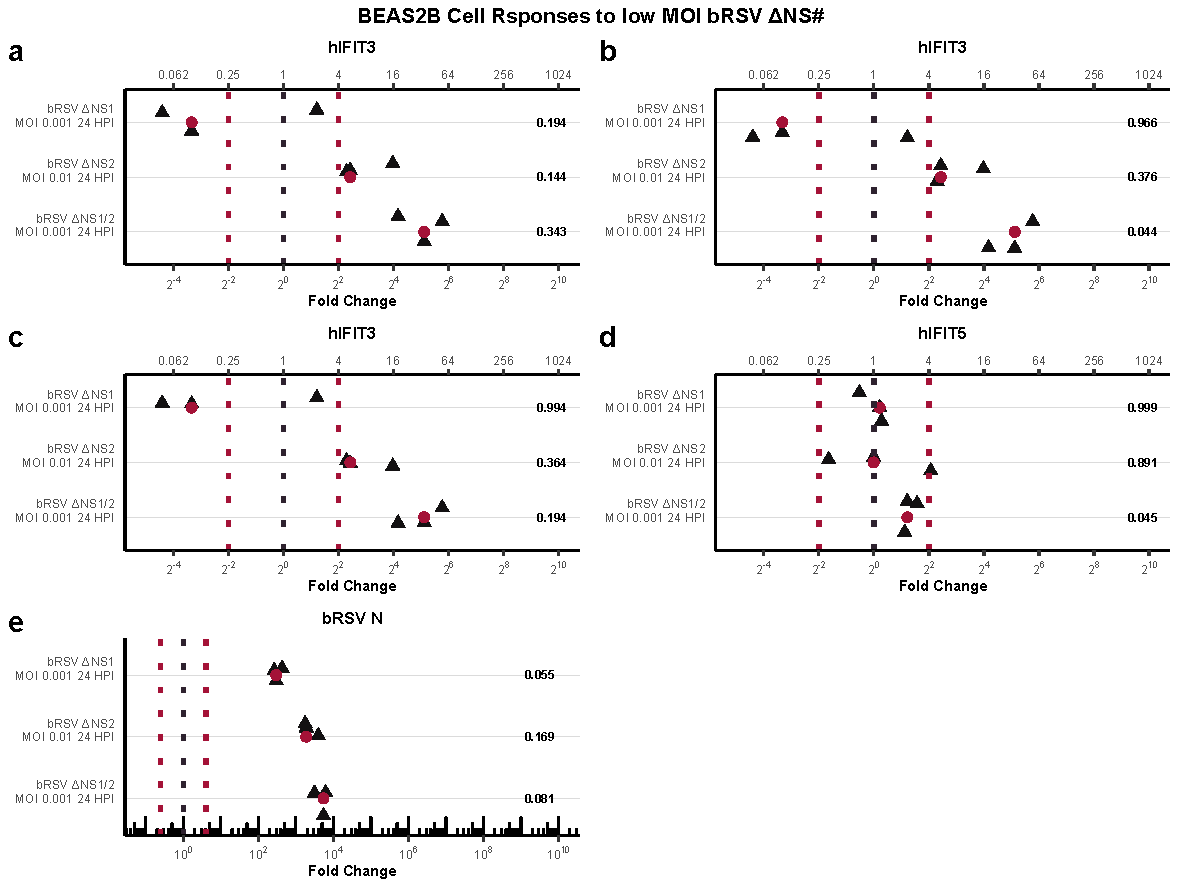
\includegraphics[width=1\linewidth]{06. Chapter 1/Figs/01. Induction/12. beas2b_brsv_dns.pdf}
    \caption[BEAS-2B responses to bRSV dNSs.]{BEAS-2B responses to bRSV dNSs.}
    \label{BEAS-2B responses to bRSV dNSs.}
\end{figure}










